
\section{Introduction}

The demands of everyday life require us to flexibly shift our attention between many different aspects of the visual world. When researchers operationalize these behaviors they often turn to tasks in which an observer must select information from the visual scene either from a spatial location or a particular feature dimension. This distinction has led to categorizing covert visual attention into two types: spatial attention, when task demands require selecting information at a specific location and not others, and feature-based attention, where task demands require selecting particular features (e.g. colors, spatial frequencies, motion directions, etc). This categorization could reflect a real physiological difference in how spatial and feature-based attention are implemented by the brain. An alternative though is that space is not privileged over other features in visual cortex, and that instead selection of information is a generic computation.

Spatial and feature-based attention have occasionally been compared to each other to evaluate how their

To relate different forms of selection we designed a set of experiments in which spatial and feature selection could be measured on the same perceptual metric. In one experiment this metric was the recall of a stimulus from working memory, and in a second a comparison of two perceptually similar stimuli. In both cases we cued observers to select two stimuli out of a set of four using either the stimulus features or spatial locations. We then model each task to estimate the underlying perceptual sensitivity in each selection condition. Our results suggest that selection is generic: perceptual sensitivity does not change according to the selection process. But, the likelihood of mistaking one stimulus for another is more likely when two stimuli are overlapping in space.

Other attempts to compare spatial and feature-based:
\citep{Liu2007-ed} - spatial is slightly faster than feature-based. 

\citep{Saenz2003-qz} - same stimulus, but attending same direction or opposite directions shows an advantage for same direction 


**PAge 98 in Pashler:
Search for a T or a green element, reporting presence and location in a N-AFC task. When detected the location can be reported, and if not correct then the probability is 1/N distributed. 
See Watson and Robson 1981
Graham 1989
See also Snyder 1972, reporting letter selected by color, more likely to make errors of spatial neighbors than far away neighbors. How to refute that if space = feature? See Nissen 1985 as well.
Tsal Lavie 1988 - 3 of each color letter, report one red + more, more likely to be neighbors than to be the same color. But is this just convenience because color vs. letter is at different levels? Same with Snyder, etc? Color vs. direction vs. space seems more reasonable test?
Carrasco paper from early 2000s


\section{Methods}

\subsection{Observers}
In total X observers were subjects for the experiments. All observers except one (who was an author) were naive to the intent of the experiments. X observers were excluded during the initial training sessions due to an inability to maintain appropriate fixation (see eye-tracking below). Procedures were approved in advance by the Stanford Institutional Review Board on human participants research and all observers gave prior written informed consent before they participated in the experiment. When necessary, observers wore corrective lenses to correct their vision to normal. Observers were filtered prior to inclusion based on self-reported color vision and tested for colour vision deficits using the Ishihara test (color-blindness.com), no additional observers had to be excluded based on the test results. 

\subsection{Hardware setup for stimulus and task control}

Visual stimuli were generated using MATLAB (The Mathworks, Inc.) and MGL \citep{Gardner2018-uq}. Stimuli were displayed on a 22.5 inch VIEWPixx LCD display (resolution of 1900x1200, refresh-rate of 120 Hz) and responses collected via keyboard. Output luminance and spectral luminance distributions were measured for the LCD display with a PR650 spectrometer (Photo Research, Inc.). The gamma table for each display was dynamically adjusted at the beginning of each trial to linearize the luminance display such that the full resolution of the 8-bit table could be used to display the maximum contrast needed. The luminance spectra were used to compute a transformation matrix from the L*a*b* color space to the RGB output of the screen, such that the a* and b* dimensions could be separately manipulated without changing the luminance (L*). Other sources of light were minimized during behavior.

\subsection{Eye tracking}

Eye-tracking was performed using an infrared video-based eye-tracker at 500 Hz (Eyelink 1000; SR Research). Calibration was performed throughout each session to maintain a validation accuracy of less than 1 degree average offset from expected using a thirteen-point calibration procedure. Trials were initiated by fixating the central cross for 300 ms and canceled on-line when an observer’s eye position moved more than 1.5 degree away from the center of the fixation cross for more than 300 ms. During training and before data collection. observers were excluded from further participation if we were unable to calibrate the eye tracker to an error of less than 1 degree of visual angle or if their canceled trial rate did not drop to near zero.

\subsection{Experimental design}

\subsubsection{Averaging task}

Stimuli consisted of two pairs of dot patches, to the left and right of a central fixation cross (0.5 x 0.5 deg). The dot patches were circular regions centered 8 degrees eccentric with a diameter of 10 deg, covering from 3 to 13 deg along the horizontal axis and -5 to +5 deg along the vertical axis. Each patch was filled with two sets of moving dots (0.2 dots / deg$^2$, per set, 0.3 deg diameter). Dots within a patch were given an identical color (equal luminance, with a* and b* varying) and moved in the same direction at 3.5 deg / s. Dots were `alive' for 0.25 s before vanishing and reappearing immediately at a new random location.

On each trial in the averaging task observers were asked to report the average motion direction of two dot patches (Fig. \ref{fig:c4f1}. Before each set of 20 trials observers were told which feature they would be selecting the patches with with the phrase ``cue side'' or ``cue color'' shown at fixation. Each trial was initiated by the observer fixating the central cross for 300 ms. This was followed by a 0.75 s cue, either a line to the left or right or a miniature patch of colored dots. The feature instructed the observers about which two dot patches they would need to average: either the two on the left, on the right, or the two yellow or blue patches (one on the left and one on the right). A 0.75 s delay followed. 

\subsubsection{Estimation task}


On each trial in the estimation task observers were asked to report about either the color or motion direction of a single dot patch. Before each block of 40 trials observers were told which feature would be reported with either the phrase ``report color'' or ``report direction'' appearing on the screen. Key to the task was that although observers ultimately reported about only one dot patch they could be cued to remember just that patch, or multiple patches, during a brief delay period. Each trial consisted of the following sequence: a fixation period

\subsection{Channel linking model}

To model the results of the estimation and averaging tasks we 

\section{Results}


\begin{figure}
\centering
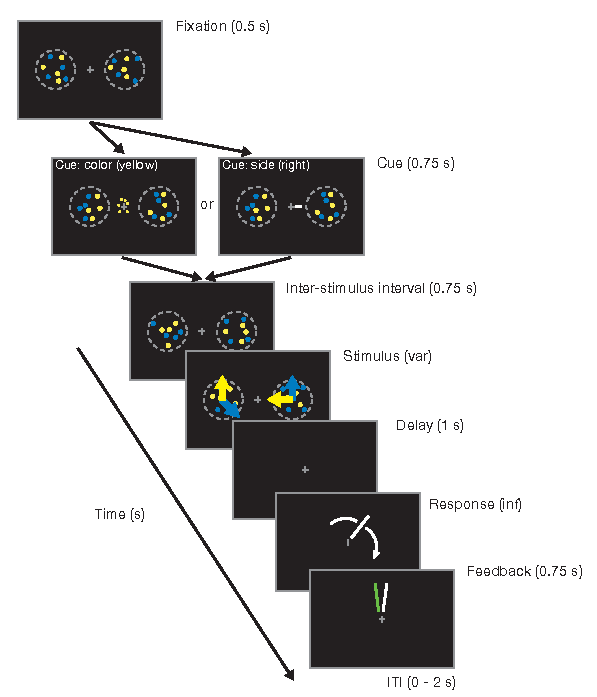
\includegraphics[keepaspectratio,width=0.5\textwidth]{figs_c4/f1_task.pdf}
\caption[Averaging task]{Averaging task}
\label{fig:c4f1}
\end{figure}


\begin{figure}
\centering
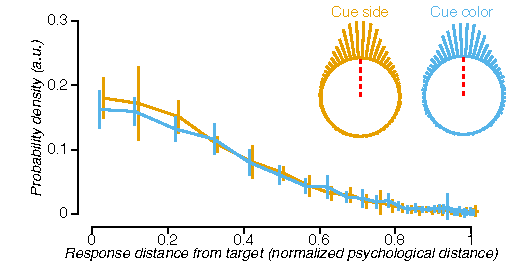
\includegraphics[keepaspectratio,width=0.5\textwidth]{figs_c4/f2_aca_perf.pdf}
\caption[Behavioral task]{}
\label{fig:c4f2}
\end{figure}


\begin{figure}
\centering
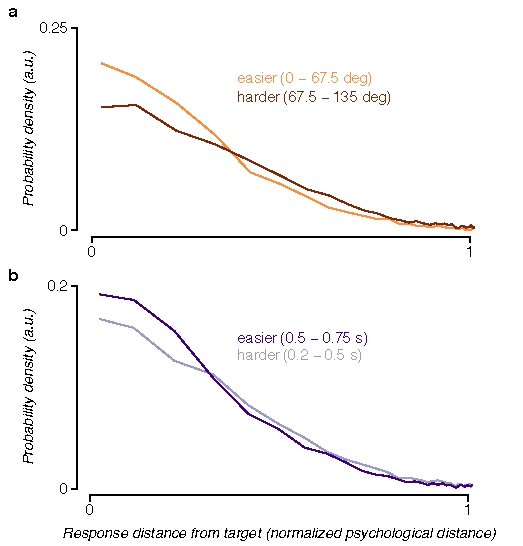
\includegraphics[keepaspectratio,width=0.5\textwidth]{figs_c4/f2_aca_parameters.pdf}
\caption[Behavioral task]{}
\label{fig:c4f3}
\end{figure}

\begin{figure}
\centering
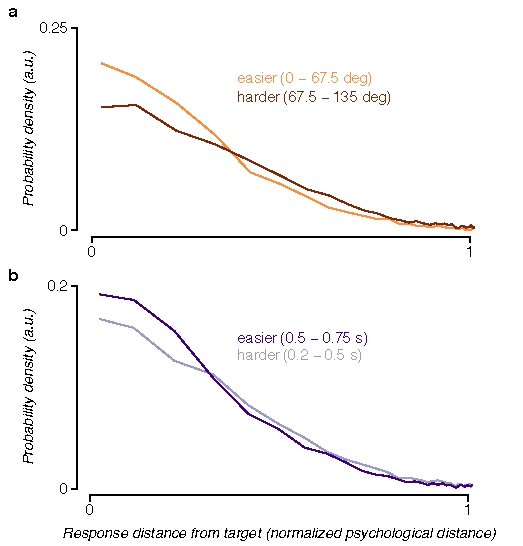
\includegraphics[keepaspectratio,width=0.5\textwidth]{figs_c4/f2_aca_parameters.pdf}
\caption[Behavioral task]{}
\label{fig:c4f3}
\end{figure}

\section{Discussion}

